%@TheDoctorRAB
%standard white paper/preproposal format
%
%%%%%
%
%REFERENCES
%
%neup.bst - numbered citations in order of appearance, short author list with et al in reference section
%nsf.bst - numbered citations in order of appearance, full author list in references section
%standard.bst - citations with author last name with et al for more than 2 authors; full author list in references section
%ans.bst is for ANS only. 
%
%author = {Lastname, Firstname and Lastname, Firstname and Lastname, Firstname} for all bst formats
%bst renders the author list itself
%
%author = {{Nuclear Regulatory Commission}} if the author is an organization, institution, etc., and not people
%
%title = {{}} for all
%
%for all - use \citep{-} - [1] or (Borrelli, 2021) in the text
%standard.bst \cite{-} - Borrelli (2021) in the text
%standard.bst lists references alphabetically
%the rest list numerically
%
%
%%% slides 
%
%\citep{xxxnna} where the citation should go
%\blfootnote{\fontsize\cite{xxxnna}\fontsize\bibentry{xxxnna}} before \end{frame}
%
%
%%%%%

%%%%% presentation settings
\documentclass[aspectratio=1610,pdftex,dvipsnames,compress,xcolor={dvipsnames}]{beamer}
\usetheme{Boadilla}
\usecolortheme{seahorse}
\beamertemplatenavigationsymbolsempty
\addtobeamertemplate{footnote}{\hskip -2em}{} %pushes footnote to margin
\setbeamerfont{title}{series=\bfseries}
\setbeamertemplate{page number in head/foot}[framenumber] %just gives slide number; comment out for 1/7, 2/7...
\definecolor{BackGround}{RGB}{255,250,240}
\setbeamercolor{background canvas}{bg=BackGround}
%%%%%


%%%%% general 
%\documentclass[11pt,a4paper]{article}
%\usepackage[lmargin=1in,rmargin=1in,tmargin=1in,bmargin=1in]{geometry}
\usepackage[pagewise]{lineno} %line numbering
\usepackage{setspace}
\usepackage{ulem} %strikethrough - do not \sout{\cite{}}
\usepackage{graphicx}
\usepackage{mypythonhighlight,verbatim}
\usepackage{filecontents}
\usepackage{tablefootnote}
\usepackage{footnotehyper}
\usepackage{float}
%\usepackage{subfig}
\usepackage[yyyymmdd]{datetime} %date format
\renewcommand{\dateseparator}{.}
\graphicspath{{img/}} %path to graphics
\setcounter{secnumdepth}{5} %set subsection to nth level
\usepackage{needspace}
\usepackage[stable,hang,flushmargin]{footmisc} %footnotes in section titles and no indent; standard.bst
\usepackage[inline]{enumitem}
\setlist[itemize]{label=\textbullet}
\usepackage{boldline}
\usepackage{makecell}
\usepackage{booktabs}
\usepackage{amssymb}
\usepackage{gensymb}
\usepackage{amsmath,nicefrac}
\usepackage{physics}
\usepackage{lscape}
\usepackage{array}
\usepackage{chngcntr}
\usepackage{hyperref}
\hypersetup{colorlinks,linkcolor=black,citecolor=black,urlcolor=blue} 
%\usepackage{sectsty}
\usepackage{textcomp}
\usepackage{lastpage}
\usepackage{xargs} %for \newcommandx
\usepackage[colorinlistoftodos,prependcaption,textsize=tiny]{todonotes} %makes colored boxes for commenting
\usepackage{soul}
\usepackage{color}
\usepackage{marginnote}
\usepackage[figure,table]{totalcount}
\usepackage[capitalise]{cleveref}
\usepackage{microtype} %improves typography for pdf
\usepackage[pdftex,dvipsnames]{colortbl} %change font color
%%%%%


%%%%% tikz
\usepackage{pgf}
\usepackage{tikz} % required for drawing custom shapes
\usetikzlibrary{shapes,arrows,automata,trees}
%%%%%


%%%%% fonts
\usepackage{times}
%arial - uncomment next two lines
%\usepackage{helvet}
%\renewcommand{\familydefault}{\sfdefault}
%%%%%


%%%%% references
%\usepackage[round,semicolon]{natbib} %for (Borrelli 2021; Clooney 2019) - standard.bst 
\usepackage[numbers,sort&compress]{natbib} %for [1-3] - nsf.bst, neup.bst
\setlength{\bibsep}{7pt} %sets space between references
%\renewcommand{\bibsection}{} %suppresses large 'references' heading
%\renewcommand\bibpreamble{\vspace{\baselineskip}} %sets spacing after heading if not using default references heading
%%%%%


%%%%% tables and figures
\usepackage{longtable} %need to put label at top under caption then \\ - use spacing
\usepackage{tablefootnote}
\usepackage{tabularx}
\usepackage{multirow}
\usepackage{tabto} %general tabbed spacing
\usepackage{pdfpages}
\usepackage{wrapfig} %wraps figures around text
\setlength{\intextsep}{0.00mm}
\setlength{\columnsep}{1.00mm}
\usepackage[singlelinecheck=false,labelfont=bf]{caption}
\usepackage{subcaption}
\captionsetup[table]{justification=justified,skip=5pt,labelformat={default},labelsep=period,name={Table}} %sets a space after table caption
\captionsetup[figure]{justification=justified,skip=5pt,labelformat={default},labelsep=period,name={Figure}} %sets space above caption, 'figure' format
\captionsetup[wrapfigure]{justification=centering,aboveskip=0pt,belowskip=0pt,labelformat={default},labelsep=period,name={Fig.}} %sets space above caption, 'figure' format
\captionsetup[wraptable]{justification=centering,aboveskip=0pt,belowskip=0pt,labelformat={default},labelsep=period,name={Table}} %sets space above caption, 'figure' format
%%%%%


%%%%% watermark
%\usepackage[firstpage,vpos=0.63\paperheight]{draftwatermark}
%\SetWatermarkText{\shortstack{DRAFT\\do not distribute}}
%\SetWatermarkScale{0.20}
%%%%%


%%%%% cross referencing files
%\usepackage{xr} %for revisions - will cross reference from one file to here
%\externaldocument{/path/to/auxfilename} %aux file needed
%%%%%


%%%%% toc and glossaries
\usepackage[toc,title]{appendix}
\usepackage[acronym,nomain,nonumberlist]{glossaries}
\makenoidxglossaries
%\usepackage{titlesec,titletoc}
%\renewcommand{\thepart}{ARTICLE \Roman{part}} %puts the label into the command so \thelabel will carry through
%\renewcommand{\thesection}{\arabic{section}} %puts the label into the command so \thelabel will carry through
%\titleformat{\part}{\normalfont\large\bfseries}{\thepart}{}{}[]
%\titlespacing*\part{0pt}{0.95\baselineskip}{0.75\baselineskip}
%\titleformat{\section}[runin]{\normalfont\large\bfseries}{\thesection}{-1em}{}[.]
%\titlespacing*\section{0pt}{0.65\baselineskip}{0.55\baselineskip}
%\titleformat{\subsection}[runin]{\normalfont\normalsize\bfseries}{\thesubsection}{-1em}{}[.]
%\titlespacing*\subsection{0pt}{0.50\baselineskip}{0.35\baselineskip}
%\titleformat{\paragraph}[runin]{\normalfont\normalsize\bfseries\itshape}{\theparagraph}{-1em}{}[.]
%\titlespacing*\paragraph{0pt}{0.45\baselineskip}{0.25\baselineskip}
%\titleformat{\subparagraph}[runin]{\normalfont\normalsize\itshape}{\thesubparagraph}{-1em}{}[.]
%\titlespacing*\subparagraph{0pt}{0.40\baselineskip}{0.25\baselineskip}
%\titleformat{\paragraph}[hang]{\normalfont\normalsize\bfseries}{\theparagraph}{5pt}{}[]
%\titlespacing*\paragraph{0pt}{0.50\baselineskip}{0.25\baselineskip}
%\titleformat{\subparagraph}[runin]{\normalfont\normalsize\itshape}{\thesubparagraph}{-1em}{}[.]
%\titlespacing*\subparagraph{0pt}{0.40\baselineskip}{0.20\baselineskip}
%%%%%


%%%%% editing
\newcommand{\edit}[1]{\textcolor{blue}{#1}} %shortcut for changing font color on revised text
\newcommand{\fn}[1]{\footnote{#1}} %shortcut for footnote tag
\newcommand*\sq{\mathbin{\vcenter{\hbox{\rule{.3ex}{.3ex}}}}} %makes a small square as a separator $\sq$
%\newcommand{\sk}[1]{\sout{#1}} %shortcut for default strikethrough - do not sk through citep
\newcommand\sk{\bgroup\markoverwith{\textcolor{red}{\rule[0.5ex]{1pt}{1pt}}}\ULon} %strikethrough with red line; not in \section{}
%\st{} does strikethrough using soul package but does not like acronyms
\newcommand{\blucell}{\cellcolor{aliceblue}} %use to shade in table cell
\newcommand{\grycekk}{\cellcolor{lightgray}} %use to shade in table cell
\newcommand{\whicell}{\cellcolor{antiquewhite}} %use to shade in table cell
%%%%%


%%%%% colors
%http://latexcolor.com/
%https://en.wikibooks.org/wiki/LaTeX/Colors#:~:text=black%2C%20blue%2C%20brown%2C%20cyan,be%20available%20on%20all%20systems.
\definecolor{aliceblue}{rgb}{0.94, 0.97, 1.0}
\definecolor{antiquewhite}{rgb}{0.98, 0.92, 0.84}
\definecolor{lightmauve}{rgb}{0.86, 0.82, 1.0}
\definecolor{brilliantlavender}{rgb}{0.96, 0.73, 1.0}
\definecolor{brandeisblue}{rgb}{0.0, 0.44, 1.0}
\definecolor{darkmidnightblue}{rgb}{0.0, 0.2, 0.4}

\newcommand{\x}{\cellcolor{aliceblue}} %use to shade in table cell
\newcommand{\y}{\cellcolor{lightgray}} %use to shade in table cell
\newcommand{\z}{\cellcolor{antiquewhite}} %use to shade in table cell
%%%%%


%%%%% acronyms
\newcommand{\acf}{\acrfull} %full acronym
\newcommand{\acl}{\acrlong} %long acronym
\newcommand{\acs}{\acrshort} %short acronym

\newcommand{\acfp}{\acrfullpl} %full acronym plural
\newcommand{\aclp}{\acrlongpl} %long acronym plural
\newcommand{\acsp}{\acrshortpl} %short acronym plural
%%%%%


%%%%% todonotes
\newcommandx{\cmt}[2][1=]{\todo[author=\textbf{STRUCTURE},tickmarkheight=0.15cm,linecolor=red,backgroundcolor=red!25,bordercolor=black,#1]{#2}}
\newcommandx{\con}[2][1=]{\todo[author=\textbf{CONTENT},tickmarkheight=0.15cm,linecolor=brilliantlavender,backgroundcolor=brilliantlavender,bordercolor=black,#1]{#2}}
\newcommandx{\rab}[2][1=]{\todo[noline,author=\textbf{RAB},backgroundcolor=Plum!25,bordercolor=black,#1]{#2}}


%\newcommandx{\jon}[2][1=]{\todo[noline,author=\textbf{ATTN: Johnson},backgroundcolor=blue!25,bordercolor=black,#1]{#2}}
%\newcommandx{\han}[2][1=]{\todo[noline,author=\textbf{ATTN: Haney},backgroundcolor=OliveGreen!25,bordercolor=black,#1]{#2}}
%\newcommandx{\rab}[2][1=]{\todo[author=\textbf{RAB},tickmarkheight=0.15cm,linecolor=Plum,backgroundcolor=Plum!25,bordercolor=black,#1]{#2}}
%\newcommandx{\han}[2][1=]{\todo[author=\textbf{ATTN: Haney},tickmarkheight=0.15cm,linecolor=OliveGreen,backgroundcolor=OliveGreen!25,bordercolor=OliveGreen,#1]{#2}}
%\newcommandx{\jon}[2][1=]{\todo[author=\textbf{ATTN: Johnson},tickmarkheight=0.15cm,linecolor=blue,backgroundcolor=blue!25,bordercolor=blue,#1]{#2}}


% highlighting 
\DeclareRobustCommand{\hlc}[1]{{\sethlcolor{LimeGreen}\hl{#1}}}
\makeatletter
    \if@todonotes@disabled
    \newcommand{\hlh}[2]{#1}
    \else
    \newcommand{\hlh}[2]{\han{#2}\hlc{#1}}
    \fi
    \makeatother

\DeclareRobustCommand{\hld}[1]{{\sethlcolor{CornflowerBlue}\hl{#1}}}
\makeatletter
    \if@todonotes@disabled
    \newcommand{\hlj}[2]{#1}
    \else
    \newcommand{\hlj}[2]{\jon{#2}\hld{#1}}
    \fi
    \makeatother

\DeclareRobustCommand{\hlf}[1]{{\sethlcolor{lightmauve}\hl{#1}}}
\makeatletter
    \if@todonotes@disabled
    \newcommand{\hlb}[2]{#1}
    \else
    \newcommand{\hlb}[2]{\rab{#2}\hlf{#1}}
    \fi
    \makeatother
%%%%%


%%%%% table alignments
\newcolumntype{L}[1]{>{\raggedright\let\newline\\\arraybackslash\hspace{0pt}}m{#1}} %uses \raggedright with m,p{} in table column
\newcolumntype{C}[1]{>{\centering\let\newline\\\arraybackslash\hspace{0pt}}m{#1}} %uses \raggedright with m,p{} in table column
\newcolumntype{R}[1]{>{\raggedleft\let\newline\\\arraybackslash\hspace{0pt}}m{#1}} %uses \raggedright with m,p{} in table column
%%%%%


%%%%% table contents
\makeatletter
\renewcommand\tableofcontents{%
    \@starttoc{toc}%
}
\makeatother

\makeatletter
\renewcommand\listoffigures{%
    \@starttoc{lof}%
}
\makeatother

\makeatletter
\renewcommand\listoftables{%
    \@starttoc{lot}%
}
\makeatother

\makeatletter
\newcommand*\ftp{\fontsize{16.5}{17.5}\selectfont}
\makeatother
%%%%%


%%%%% user commands
\newcommand\blfootnote[1]{%
  \begingroup
  \renewcommand\thefootnote{}\footnote{#1}%
  \addtocounter{footnote}{-1}%
  \endgroup
}

\makeatletter
\renewcommand{\@biblabel}[1]{#1.\hfill} %bibliography ordered list has numbers left flush
\makeatother
%%%%%

%%%%% archived section commands - use titlesec
%\makeatletter
%\renewcommand\section{%
%    \@startsection{section}{1}{\z@ }{0.50\baselineskip}{0.25\baselineskip}
%    {\large \normalfont \bfseries}}%

%\makeatletter
%\renewcommand\paragraph{%
%    \@startsection{paragraph}{4}{\z@ }{0.55\baselineskip}{-1em}
%    {\normalfont \normalsize \bfseries}}%

%\makeatletter
%\renewcommand\subparagraph{%
%    \@startsection{subparagraph}{5}{\z@ }{0.40\baselineskip}{-1em}
%    {\normalfont \normalsize \itshape }}%

%\makeatletter
%\renewcommand\subsection{%
%    \@startsection{subsection}{2}{\z@ }{0.45\baselineskip}{0.25\baselineskip}
%    {\large \normalfont \bfseries}}%
%%%%%


%%%%% header and footer
%\usepackage{fancyhdr}
%\pagestyle{fancy}
%\fancyhf{} %move page number to bottom right
%\renewcommand{\headrulewidth}{0pt} %set line thickness in header; uncomment as is to remove line
%\lhead{\scriptsize Name}
%\lhead{\scriptsize PNUCENE-D-22-xxxxx}
%\chead{\scriptsize \textit{PhD White Paper Project Proposal}}
%\rhead{\scriptsize \today}
%\rfoot{\thepage}
%%%%%


%%%%%%% citations
%\begin{filecontents}{references.bib}
%\end{filecontents}
%%%%%%%


%%%%% acronyms
% alphabetical ordering is automated
\newacronym{nrs}{NRHES}{Nuclear Renewable Hybrid Energy System}
\newacronym{ahp}{AHP}{Analytical Hierarchy Process}
\newacronym{inl}{INL}{Idaho National Laboratory}
\newacronym{orl}{ORNL}{Oak Ridge National Laboratory}
\newacronym{anl}{ANL}{Argonne National Laboratory}
\newacronym{npp}{NPP}{Nuclear Power Plant}
\newacronym{smr}{SMR}{Small Modular Reactor}
\newacronym{ump}{UAMPS}{Utah Associated Municipal Power Systems}
\newacronym{nus}{NuScale}{NuScale Power, LLC}
\newacronym{nrc}{NRC}{United States Nuclear Regulatory Commission}
\newacronym{epri}{EPRI}{Electric Power Research Institute}
\newacronym{nerc}{NERC}{North American Electric Reliability Corporation}
\newacronym{ci}{CI}{Consistency Index}
\newacronym{cr}{CR}{Consistency Ratio}
\newacronym{htse}{HTSE}{High Temperature Steam Electrolysis}
\newacronym{lwr}{LWR}{Light Water Reactor}
\newacronym{eia}{EIA}{U.S. Energy Information Administration}
\newacronym{oer}{OER}{Online Educational Resource}
\newacronym{lms}{LMS}{Learning Management System}
\newacronym{cps}{CPS}{Cyber-Physical Systems}
\newacronym{nsf}{NSF}{National Science Foundation}
\newacronym{wsc}{WSC}{Western Services Corporation}
\newacronym{cae}{CAES}{Center for Advanced Energy Studies}
\newacronym{hsl}{HSSL}{Human System Simulation Laboratory}
\newacronym{pwr}{PWR}{Pressurized Water Reactor}
\newacronym{bwr}{BWR}{Boiling Water Reactor}
\newacronym{roi}{ROI}{Return on Investment}
\newacronym{ic}{I\&C}{Instrumentation \& Controls}
\newacronym{mwe}{MWe}{Megawatts-electric}
\newacronym{ics}{ICS}{Industrial Control Systems}
\newacronym{sca}{SCADA}{Supervisory Control and Data Acquisition}
\newacronym{ip}{IP}{Internet Protocol}
\newacronym{udp}{UDP}{User Datagram Protocol}
\newacronym{tva}{TVA}{Tennessee Valley Authority}
\newacronym{plc}{PLC}{Programmable Logic Controller}
\newacronym{vfd}{VFD}{Variable Frequency Drive}
\newacronym{khp}{KHNP}{Korean Hydro \& Nuclear Power Co., Ltd}
\newacronym{onl}{ORNL}{Oak Ridge National Laboratory}
\newacronym{jcp}{JCPOA}{Joint Comprehensive Plan of Action}
\newacronym{mim}{MITM}{Man in the Middle}
\newacronym{dos}{DDoS}{Distributed Denial of Service}
\newacronym{tcp}{TCP/IP}{Transmission Control Protocol/Internet Protocol}
\newacronym{dnp}{DNP3}{Distributed Network Protocol 3}
\newacronym{pra}{PRA}{Probabilistic Risk Assessment}
\newacronym{cs}{CS}{Critical System}
\newacronym{loc}{LOCA}{Loss of Coolant Accident}
\newacronym{hmi}{HMI}{Human Machine Interface}
\newacronym{pha}{PHA}{Preliminary Hazards Analysis}
\newacronym{bol}{BOL}{Beginning-of-Life}
\newacronym{eol}{EOL}{End-of-Life}
\newacronym{mol}{MOL}{Middle-of-Life}
\newacronym{imu}{IMUNES}{Integrated Multiprotocol Network Emulator/Simulator}
\newacronym{ccc}{CCC}{Computing Community Consortium}
\newacronym{neu}{NEUP}{Nuclear Energy University Program}
\newacronym{doe}{DOE}{United States Department of Energy}
\newacronym{nei}{NEI}{Nuclear Energy Institute}
\newacronym{nit}{NITRD}{Networking Information Technology Research \& Development Program}
\newacronym{rcs}{RCS}{Reactor Cooling System}
\newacronym{con}{IC}{Initial Condition}
\newacronym{csi}{CSIS}{Center for Strategic \& International Studies}
\newacronym{pcap}{PCAP}{packet capture file}
\newacronym{dc}{DC}{Direct-Current}
\newacronym{ac}{AC}{Alternating-Current}
\newacronym{iff}{UIIF}{Idaho Falls Center for Higher Education}
\newacronym{snl}{SNL}{Sandia National Laboratory}
\newacronym{cie}{CIE}{Cyber-Informed Engineering}
\newacronym{cds}{CRDS}{Control Rod Drive System}
\newacronym{cdm}{CRDM}{Control Rod Drive Mechanism}
\newacronym{fma}{FMEA}{Failure Modes \& Effects Analysis}
\newacronym{rpn}{RPN}{Risk Priority Number}
\newacronym{scr}{SCR}{silicon controller rectifier}
\newacronym{hvc}{HVAC}{Heating, Ventilation \& Air Conditioning}
\newacronym{ttb}{TTB}{Time-to-Boil}
\newacronym{sis}{SIS}{Safety Instrumented System}
\newacronym{ui}{UI}{University of Idaho}
\newacronym{ke}{KE}{Kinetic Energy}
%\newacronym{}{}{}
%%%%%

%%%%% spacing
%\onehalfspacing %linespacing
%\setstretch{1.05} %linespacing
%\spacing{1.25} %equivalent to 1.5 line spacing in Word
%%%%%


%%%%% linenumbering
%\linenumbers %toggle line numbers
%\pagewiselinenumbers %reset line numbers on new page
%\modulolinenumbers[1] %line numbering interval
%%%%%


%%%%% title page
\addtocounter{framenumber}{-1} %does not count the title slide in the slide count
\title[NE585 - Nuclear fuel cycles]{NE585\\NUCLEAR FUEL CYCLES\\Interaction of radiation with matter\\2}
\author[@TheDoctorRAB]{R. A. Borrelli}
\institute[]{
    \acl{ui}\\
    \vspace{0.10in}
    
\includegraphics[width=0.20\textwidth]{ne-logo.png}
    }
\date{\acl{iff}}
%%%%%


\begin{document}


%%%%% title page with no footer
{
    \setbeamertemplate{footline}{}
    \begin{frame}
        \titlepage
    \end{frame}
}
%%%%%


\begin{frame}{Learning objectives}
    \begin{enumerate}[series=outerlist,topsep=0pt,itemsep=21pt,leftmargin=*,label=(\arabic*)]
        \item[]Explain the different ways radiation interacts with matter
        \item[]Apply the concept of cross sections to neutron interactions with matter
        \item[]Derive neutron scattering relationships
        \item[]Book -- Chapter 3
    \end{enumerate}
\end{frame}


\begin{frame}{Learning nodes}
    \begin{columns}[t]

        \begin{column}{0.50\textwidth}
            \begin{enumerate}[series=outerlist,topsep=0pt,itemsep=1pt,leftmargin=*,label=(\arabic*)]
                \item[]\textbf{Gamma ray interactions}
                \item[]Photoelectric effect
                \item[]Pair production
                \item[]Compton effect
                    \vspace{0.15in}
                \item[]\textbf{Fission}
                    \vspace{0.15in}
                \item[]\textbf{Neutron interactions}
                \item[]Elastic scattering
                \item[]Lethargy
                \item[]Inelastic scattering
                \item[]Radiative capture
                \item[]Charged particle emission
                \item[]Bremsstrahlung radiation
            \end{enumerate}
        \end{column}

        \begin{column}{0.50\textwidth}
            \begin{enumerate}[series=outerlist,topsep=0pt,itemsep=1pt,leftmargin=*,label=(\arabic*)]
                \item[]\hfill\textbf{Cross sections}
                    \vspace{0.15in}
                \item[]\hfill\textbf{Neutron density}
                    \vspace{0.15in}
                \item[]\hfill\textbf{Neutron fluence}
                    \vspace{0.15in}
                \item[]\hfill\textbf{Neutron flux}
            \end{enumerate}
        \end{column}

    \end{columns}
\end{frame}


\begin{frame}[plain]{}
    \centering\Large\textbf{Gamma rays interact with matter in very complicated ways}\\
    \centering\small\textbf{Fortunately for us we only need to know three}
\end{frame}


\begin{frame}[plain]{}
    \centering\LARGE\textbf{Photoelectric effect}
\end{frame}


\addtocounter{framenumber}{-2} 
\begin{frame}{The photoelectric effect occurs when a high energy photon knocks out an electron}
    \begin{enumerate}[series=outerlist,topsep=0pt,itemsep=21pt,leftmargin=*,label=(\arabic*)]
        \item[]Interacts with entire atom
        \item[]Electron ejected
        \item[]Leaves a positively charged ion
        \item[]Usually an x ray emission
        \item[]Atom recoil carries little \acf{ke}
        \item[]Highly probable with heavier atoms
        \item[]Why?
    \end{enumerate}
\end{frame}


\begin{frame}{}
    \begin{figure}
        \centering
        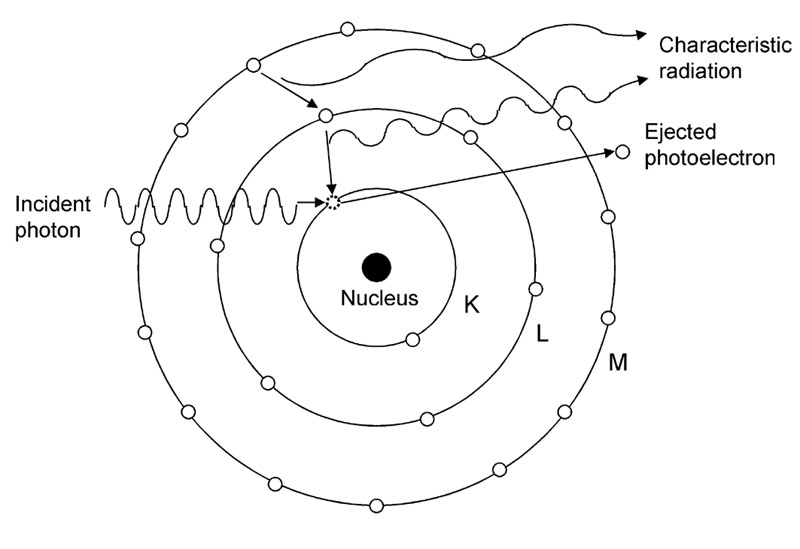
\includegraphics[width=0.95\textwidth]{pe.jpg}
%        \caption{}
    \end{figure}
\end{frame}


\begin{frame}[plain]{}
    \centering\LARGE\textbf{Pair production}
\end{frame}


\addtocounter{framenumber}{-1} 
\begin{frame}{For pair production, a high energy photon creates a negatron and positron}
    \begin{enumerate}[series=outerlist,topsep=0pt,itemsep=21pt,leftmargin=*,label=(\arabic*)]
        \item[]Only occurs with photon above $1.022 \; MeV$
        \item[]And near the nucleus
        \item[]Why?
        \item[]Then they react with other negatrons/positrons
        \item[]Give off characteristic $0.511 \; MeV$ photons
        \item[]Only in vicinity of Coulomb field
    \end{enumerate}
\end{frame}


\begin{frame}{}
    \begin{figure}
        \centering
        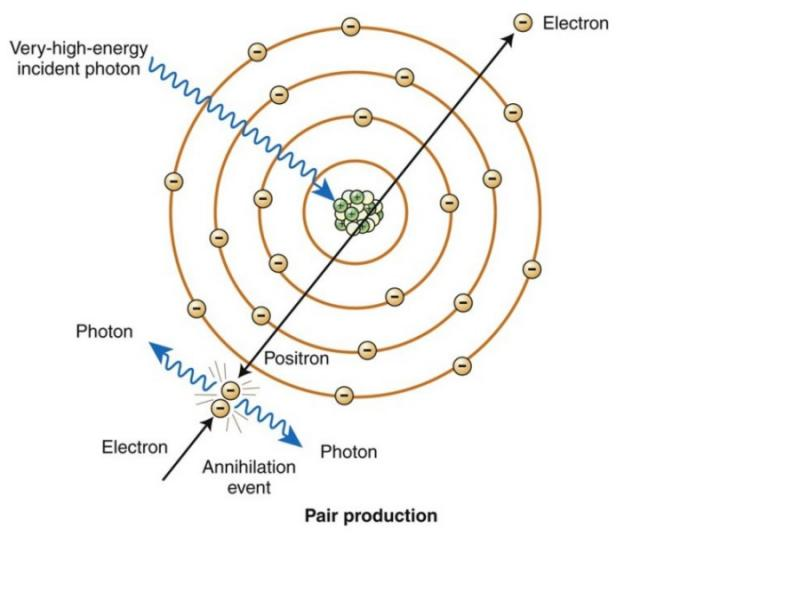
\includegraphics[width=0.75\textwidth]{pp.jpg}
%        \caption{}
    \end{figure}
\end{frame}


\begin{frame}[plain]{}
    \centering\LARGE\textbf{Compton effect}
\end{frame}


\addtocounter{framenumber}{-1} 
\begin{frame}{The Compton effect is elastic scattering of a photon by an electron}
    \begin{enumerate}[series=outerlist,topsep=0pt,itemsep=21pt,leftmargin=*,label=(\arabic*)]
        \item[]Energy and momentum are conserved
        \item[]All angles of scattering possible
    \end{enumerate}

    \begin{equation}
        \LARGE
        E_2 = \frac{E_1 E_{\epsilon}}{E_1 (1 - cos \theta) + E_{\epsilon}}
    \end{equation}

    \vspace*{\fill}

    \begin{enumerate}[series=outerlist,topsep=0pt,itemsep=21pt,leftmargin=*,label=(\arabic*)]
        \item[]Should be able to derive maximum energy from this equation
        \item[]Why would the Compton effect cause problems with shielding?
            \footnote[frame]{\tiny(Talk about NE class experiment at WPI)}
    \end{enumerate}
\end{frame}


\begin{frame}{}
    \begin{figure}
        \centering
        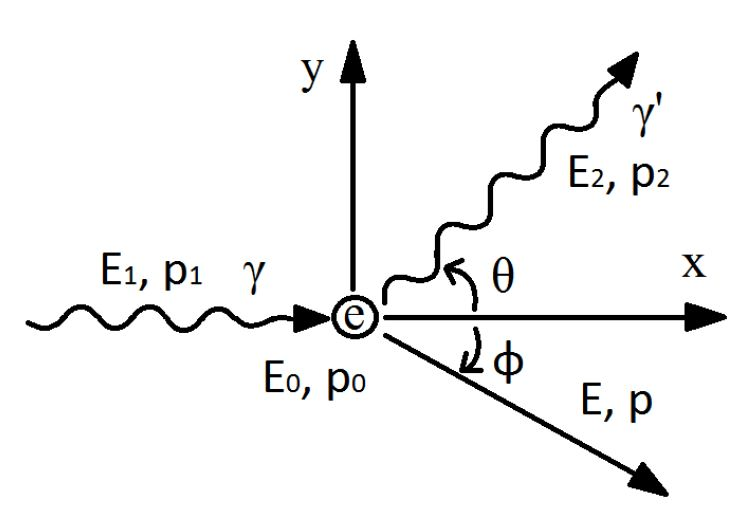
\includegraphics[width=0.75\textwidth]{scattering.jpg}
%        \caption{}
    \end{figure}
\end{frame}


\begin{frame}[plain]{}
    \centering\LARGE\textbf{Fission}
\end{frame}


\addtocounter{framenumber}{-1} 
\begin{frame}{What is the energy of fission from thorium and uranium fuel cycles?}

    \begin{equation}
        \LARGE
        ^1_0n + ^{235}_{92}U \rightarrow ^{92}_{36}Kr + ^{141}_{56}Ba + ^1_0n + ^1_0n + ^1_0n  
    \end{equation}

    \begin{equation}
        \LARGE
        ^1_0n + ^{233}_{92}U \rightarrow ^{92}_{36}Kr + ^{141}_{56}Ba + ^1_0n   
    \end{equation}

    \begin{equation}
        \LARGE
        Q = 173.3 \; MeV, \; 185.4 \; MeV
    \end{equation}

    \vspace*{\fill}

    \begin{enumerate}[series=outerlist,topsep=0pt,itemsep=21pt,leftmargin=*,label=(\arabic*)]
        \item[]For comparison, burning a carbon atom releases 4 eV
        \item[]Some super heavy nuclei fission spontaneously
    \end{enumerate}
\end{frame}


\begin{frame}{Fission is the splitting of atoms, which releases a lot of energy}
    \begin{figure}
        \centering
        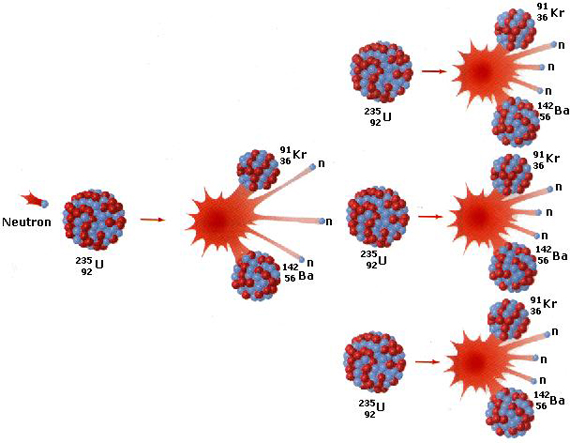
\includegraphics[width=0.55\textwidth]{fission.jpg}
%        \caption{}
    \end{figure}
\end{frame}


\begin{frame}[plain]{}
    \centering\LARGE\textbf{Neutron interactions}
\end{frame}


\addtocounter{framenumber}{-1} 
\begin{frame}{What is the energy of fission from thorium and uranium fuel cycles?}
    \begin{enumerate}[series=outerlist,topsep=0pt,itemsep=21pt,leftmargin=*,label=(\arabic*)]
        \item[]Why?
    \end{enumerate}

    \vspace*{\fill}

    \begin{equation}
        \LARGE
        ^1_0n + ^{233}_{92}U \rightarrow ^{236}_{92}U^{*} \rightarrow   
    \end{equation}

    \vspace*{\fill}

    \begin{enumerate}[series=outerlist,topsep=0pt,itemsep=21pt,leftmargin=*,label=(\arabic*)]
        \item[]Sometimes the compound nucleus is left in an excited state, before the reaction proceeds, but this can be a very short time
        \item[]What happens is highly dependent on neutron energy/temp
        \item[]So you do not always write the compound nucleus in the reaction expression
    \end{enumerate}
\end{frame}


\begin{frame}{}
    \begin{figure}
        \centering
        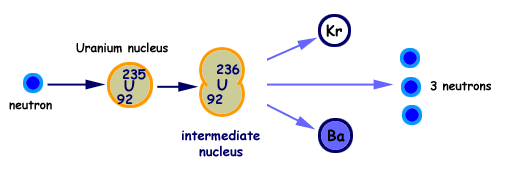
\includegraphics[width=0.75\textwidth]{compound.jpg}
%        \caption{}
    \end{figure}
\end{frame}


\begin{frame}{There are several ways neutrons interact with nuclei}
    \begin{enumerate}[series=outerlist,topsep=0pt,itemsep=21pt,leftmargin=*,label=(\arabic*)]
        \item Elastic scattering (probably most important)
        \item Inelastic scattering
        \item Radiative capture/neutron absorption
        \item Charged-particle reactions
        \item Neutron producing reactions
    \end{enumerate}
\end{frame}


\begin{frame}{What is the energy of fission from thorium and uranium fuel cycles?}

    \begin{equation}
        \LARGE
        ^1_0n + ^{233}_{92}U \rightarrow ^{236}_{92}U^{*} \rightarrow ^{233}_{92}U + ^1_0n 
    \end{equation}

    \begin{equation}
        \LARGE
        ^1_0n + ^{233}_{92}U \rightarrow ^{236}_{92}U^{*} \rightarrow ^{233}_{92}U + ^1_0n^{'}
    \end{equation}

    \begin{equation}
        \LARGE
        ^1_0n + ^{233}_{92}U \rightarrow ^{236}_{92}U^{*} \rightarrow ^{233}_{92}U + \gamma   
    \end{equation}

    \begin{equation}
        \LARGE
        ^1_0n + ^{233}_{92}U \rightarrow ^{236}_{92}U^{*} \rightarrow ^{233}_{92}U + ^{4}_{2}\alpha   
    \end{equation}

    \begin{equation}
        \LARGE
        ^1_0n + ^{233}_{92}U \rightarrow ^{236}_{92}U^{*} \rightarrow ^{233}_{92}U + 2^1_0n  
    \end{equation}

\end{frame}


\begin{frame}[plain]{}
    \centering\LARGE\textbf{Elastic scattering}
\end{frame}


\addtocounter{framenumber}{-1} 
\begin{frame}{With elastic scattering, the neutron strikes the nucleus, and they scatter}
    \begin{enumerate}[series=outerlist,topsep=0pt,itemsep=21pt,leftmargin=*,label=(\arabic*)]
        \item[]If you’ve ever played pool (billiards), it’s that sort of
        \item[]But the neutron is a lot smaller than the nucleus
        \item[]Kinetic energy and momentum is conserved with nucleus and neutron
        \item[]Nucleus can be at rest or moving, but neutron velocity is really faster
        \item[]So basically the nucleus is `at rest'
    \end{enumerate}
\end{frame}


\begin{frame}{With elastic scattering, the neutron strikes the nucleus, and they scatter}
    \begin{figure}
        \centering
        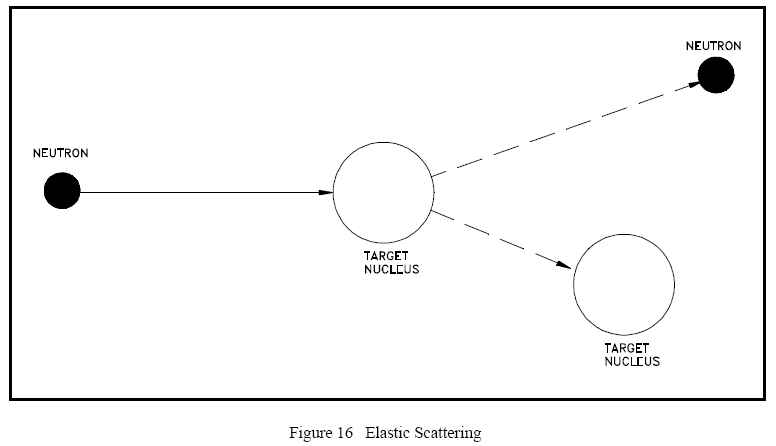
\includegraphics[width=0.75\textwidth]{neutron.elastic.scattering.jpg}
%        \caption{}
    \end{figure}
\end{frame}


\begin{frame}{The neutron energy after the collision can be obtained by conservation principles}
    \begin{columns}[t]

        \begin{column}{0.40\textwidth}
            \begin{figure}
                \centering
                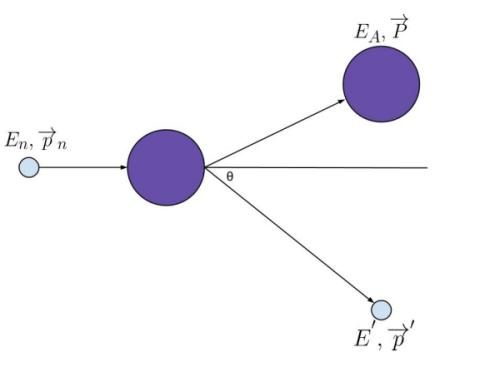
\includegraphics[width=0.95\textwidth]{neutron.elastic.scattering2.jpg}
                %\caption{}
            \end{figure}
        \end{column}

        \begin{column}{0.60\textwidth}

            \begin{equation}
                \Large
                E = E^{'} + E_A
            \end{equation}

            \begin{equation}
                \Large
                \vec{p} = \vec{p}^{'} + \vec{P}
            \end{equation}

            \begin{equation}
                \Large
                E^{'} = \frac{E_n}{(A+1)^2} \cdot [cos \theta \sqrt{A^2 - sin^2 \theta}]^2
            \end{equation}

            \begin{equation}
                \Large
                \alpha \equiv (\frac{A - 1}{A + 1})^2
            \end{equation}

            \vspace*{\fill}

            \begin{enumerate}[series=outerlist,topsep=0pt,itemsep=21pt,leftmargin=*,label=(\arabic*)]
                \item[](p58-9) - but in any edition
            \end{enumerate}
        \end{column}

    \end{columns}
\end{frame}


\begin{frame}[plain]{}
    \centering\LARGE\textbf{Lethargy}
\end{frame}


\addtocounter{framenumber}{-1} 
\begin{frame}{The concept of lethargy was invented for neutron moderation}
    \begin{enumerate}[series=outerlist,topsep=0pt,itemsep=21pt,leftmargin=*,label=(\arabic*)]
        \item[]They aren't good at naming things
    \end{enumerate}

    \vspace*{\fill}

    \begin{equation}
        \LARGE
        u \equiv ln \frac{E_M}{E}
    \end{equation}

    \vspace*{\fill}

    \begin{enumerate}[series=outerlist,topsep=0pt,itemsep=21pt,leftmargin=*,label=(\arabic*)]
        \item[]$E_M$ is the highest neutron energy in the system
        \item[]What is happening mathematically?
    \end{enumerate}
\end{frame}


\begin{frame}{The concept of lethargy was invented for neutron moderation}
    \begin{enumerate}[series=outerlist,topsep=0pt,itemsep=21pt,leftmargin=*,label=(\arabic*)]
        \item[]So, lethargy increases when neutron slows down
        \item[]Log scale is used because neutrons have huge energy range
    \end{enumerate}
\end{frame}


\begin{frame}{What we really want is average log energy loss per elastic scatter/collision}

    \begin{equation}
        \LARGE
        \xi \equiv 1 + \frac{\alpha}{1 - \alpha}ln \alpha
    \end{equation}

    \begin{equation}
        \LARGE
        \alpha \equiv (\frac{A - 1}{A + 1})^2
    \end{equation}

    \vspace*{\fill}

    \begin{enumerate}[series=outerlist,topsep=0pt,itemsep=21pt,leftmargin=*,label=(\arabic*)]
        \item[]Average change in lethargy
        \item[]What does this tell us?
        \item[]In terms of thermal reactor design?
    \end{enumerate}
\end{frame}


\begin{frame}{Because elastic scattering can be applied to find out how a neutron will slow down}

    \begin{equation}
        \LARGE
        \overline{n}_{COL} \equiv \frac{1}{\xi} ln \frac{E_1}{E_2}
    \end{equation}

    \vspace*{\fill}

    \begin{enumerate}[series=outerlist,topsep=0pt,itemsep=21pt,leftmargin=*,label=(\arabic*)]
        \item[]What is the physical interpretation?
        \item[]Moderation = getting high energy neutrons to low energy
        \item[]This means from fast moving to slow
        \item[]Why? This is a very fundamental reactor design constraint
    \end{enumerate}
\end{frame}


\begin{frame}[plain]{}
    \centering\LARGE\textbf{Inelastic scattering}
\end{frame}


\addtocounter{framenumber}{-1} 
\begin{frame}{With inelastic scattering, it is the same as elastic, but the nucleus is left in excited state}
    \begin{columns}[t]

        \begin{column}{0.50\textwidth}
            \begin{figure}
                \centering
                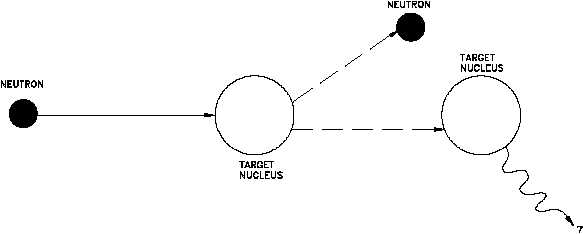
\includegraphics[width=0.95\textwidth]{inelastic.scattering.jpg}
                %\caption{}
            \end{figure}
        \end{column}

        \begin{column}{0.50\textwidth}
            \begin{enumerate}[series=outerlist,topsep=0pt,itemsep=12pt,leftmargin=*,label=(\arabic*)]
                \item[]Energy is lower for heavier nuclei
                \item[]Kinetic energy and momentum not conserved
                \item[]Compound nucleus emits lower energy neutron
                \item[]Then the nucleus emits gamma rays
                \item[]Occurs above a certain neutron energy for each nucleus
                \item[]A neutron with same energy may not scatter with different nuclei
            \end{enumerate}
        \end{column}

    \end{columns}
\end{frame}


\begin{frame}[plain]{}
    \centering\LARGE\textbf{Radiative capture}
\end{frame}


\addtocounter{framenumber}{-1} 
\begin{frame}{Because elastic scattering can be applied to find out how a neutron will slow down}
    \begin{enumerate}[series=outerlist,topsep=0pt,itemsep=21pt,leftmargin=*,label=(\arabic*)]
        \item[]This is important with reactor design (fission and fusion)
        \item[]Take a guess why?
        \item[]We also call this neutron absorption in this context
        \item[]Usually a low energy neutron reaction (why?)
        \item[]Depends on neutron energy and material
        \item[]Other applications include NAA, isotope production
    \end{enumerate}
\end{frame}


\begin{frame}{}
    \begin{figure}
        \centering
        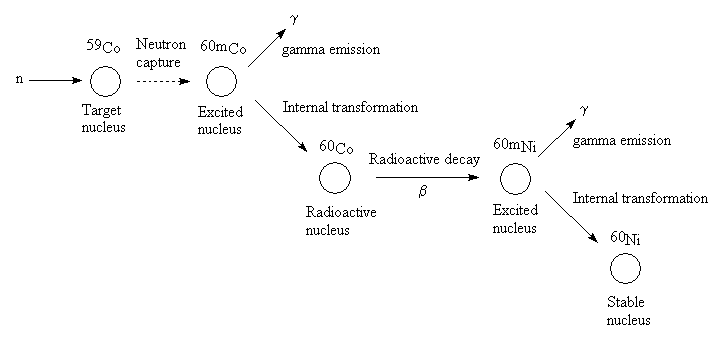
\includegraphics[width=0.75\textwidth]{capture.jpg}
%        \caption{}
    \end{figure}
\end{frame}


\begin{frame}[plain]{}
    \centering\LARGE\textbf{Charged particle emission}
\end{frame}


\addtocounter{framenumber}{-1} 
\begin{frame}{The nucleus can also absorb a neutron and emit a charged particle}
    \begin{enumerate}[series=outerlist,topsep=0pt,itemsep=21pt,leftmargin=*,label=(\arabic*)]
        \item[]This can be used to design neutron detectors
        \item[]Part of fusion reactions
        \item[]Boron is used as neutron `poison' and can absorb low energy 
        \item[]Materials testing for fuel cladding (fusion and fission)
        \item[]Charged particle production could be adverse
        \item[]Neutron depth profiling; surface of semiconductors, etc.
    \end{enumerate}

    \vspace*{\fill}

    \begin{equation}
        \LARGE
        ^{1}_{0}n + ^{10}_{5}B \rightarrow {11}_{5}B^{*} \rightarrow ^{7}_{3}Li + \alpha + \gamma
    \end{equation}

\end{frame}


\begin{frame}[plain]{}
    \centering\LARGE\textbf{Bremsstrahlung radiation}
\end{frame}


\addtocounter{framenumber}{-1} 
\begin{frame}{A consequence of charged particle reactions is the Bremsstrahlung radiation}
    \begin{enumerate}[series=outerlist,topsep=0pt,itemsep=21pt,leftmargin=*,label=(\arabic*)]
        \item[]Deceleration of the charged particle through matter
        \item[]A photon is emitted from interaction with the electron cloud or nucleus with the charged particle
        \item[]The moving particle loses energy and this is in the form of a photon
        \item[]aka `braking radiation'
        \item[]Continuous radiation distribution
        \item[]Can be used to identify galaxy clusters
        \item[]Only one page in the text but it is important to know
    \end{enumerate}
\end{frame}


\begin{frame}[plain]{}
    \centering\LARGE\textbf{Cross sections}
\end{frame}


\addtocounter{framenumber}{-1} 
\begin{frame}{A cross section tells us basically the probability of an interaction (with something)}
    \begin{enumerate}[series=outerlist,topsep=0pt,itemsep=21pt,leftmargin=*,label=(\arabic*)]
        \item[]Neutrons for us
        \item[]Cross sections for other events like Compton, etc.
        \item[]People dedicate careers to establishing precise cross sections (and good for them)
        \item[]Cross sections are given as a hypothetical area  around the target nucleus (big area, high probability)
    \end{enumerate}

    \vspace*{\fill}

    \begin{equation}
        \LARGE
        1 \; b = 10^{-24} \; cm^2
    \end{equation}

    \vspace*{\fill}

    \begin{enumerate}[series=outerlist,topsep=0pt,itemsep=21pt,leftmargin=*,label=(\arabic*)]
        \item[]Dependent on speed/energy/temperature
    \end{enumerate}
\end{frame}


\begin{frame}{Try to think of this as the likelihood of interaction}
    \begin{columns}[t]

        \begin{column}{0.40\textwidth}
            \begin{figure}
                \centering
                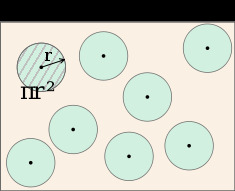
\includegraphics[width=0.95\textwidth]{cross.section.jpg}
                %\caption{}
            \end{figure}
        \end{column}

        \begin{column}{0.60\textwidth}
            \begin{enumerate}[series=outerlist,topsep=0pt,itemsep=21pt,leftmargin=*,label=(\arabic*)]
                \item[]Since there is a lot of space in between nuclei, some neutrons just fly by
                \item[]Radius of a nucleus $\sim 10^{-12} \; cm^2$, so cross section is $\sim 10^{-24} \; cm^2$  
                \item[]Which is where they derived barns
                \item[]Probability of interaction is the ratio of the total surface area of the atoms to the total area of the medium
            \end{enumerate}
        \end{column}

    \end{columns}
\end{frame}


\begin{frame}[plain]{}
    \centering\Large\textbf{How does cross section vary with temperature?}\\
    \centering\small\textbf{What is physically happening?}
\end{frame}


\addtocounter{framenumber}{-1} 
\begin{frame}{Fission cross sections have this general trend}
    \begin{columns}

        \begin{column}{0.60\textwidth}
            \begin{figure}
                \centering
                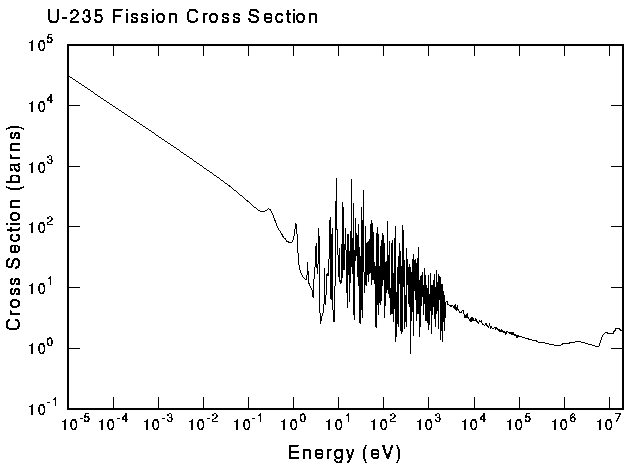
\includegraphics[width=0.95\textwidth]{u235.fission.cross.section.jpg}
                %\caption{}
            \end{figure}
        \end{column}

        \begin{column}{0.40\textwidth}
            \begin{enumerate}[series=outerlist,topsep=0pt,itemsep=21pt,leftmargin=*,label=(\arabic*)]
                \item[]If fission neutrons start at 2 MeV, where would you want them for a reactor?
            \end{enumerate}
        \end{column}

    \end{columns}
\end{frame}


\begin{frame}[plain]{}
    \centering\LARGE\textbf{Neutron density}
\end{frame}


\addtocounter{framenumber}{-1} 
\begin{frame}{Neutron density in the thermal region follows Maxwellian distribution}
    \begin{enumerate}[series=outerlist,topsep=0pt,itemsep=21pt,leftmargin=*,label=(\arabic*)]
        \item[]As fast neutrons slow down, they eventually come into thermal equilibrium with the thermal motion of the atoms in the medium through which they are moving
        \item[]Also call the $\frac{1}{v}$ region
        \item[]Resonances occur if the compound nucleus is produced in one of its characteristic excited states
        \item[]And the fast end is a smooth region
    \end{enumerate}
\end{frame}


\begin{frame}{What we really want is average log energy loss per elastic scatter/collision}

    \begin{equation}
        \LARGE
        n(E) = n_0 \frac{2\pi\sqrt{E}}{(\pi kT)^{\frac{3}{2}}} \cdot e^{-\frac{E}{kT}}
    \end{equation}

    \vspace*{\fill}

    \begin{equation}
        \LARGE
        n(v) = n_0 \frac{4\pi v^2}{(\frac{2\pi kT}{m})^{\frac{3}{2}}} \cdot e^{-\frac{mv^2}{2kT}}
    \end{equation}

\end{frame}


\begin{frame}{How does this affect reactor operation?}
    \begin{figure}
        \centering
        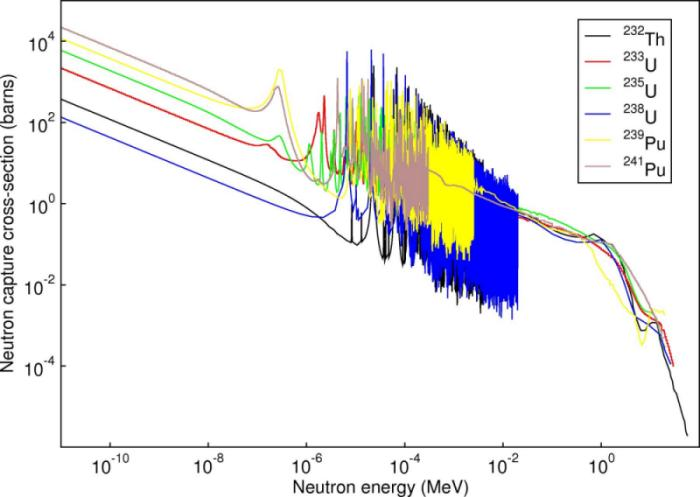
\includegraphics[width=0.75\textwidth]{capture.cross.section.jpg}
%        \caption{}
    \end{figure}
\end{frame}


\begin{frame}{}
    \begin{figure}
        \centering
        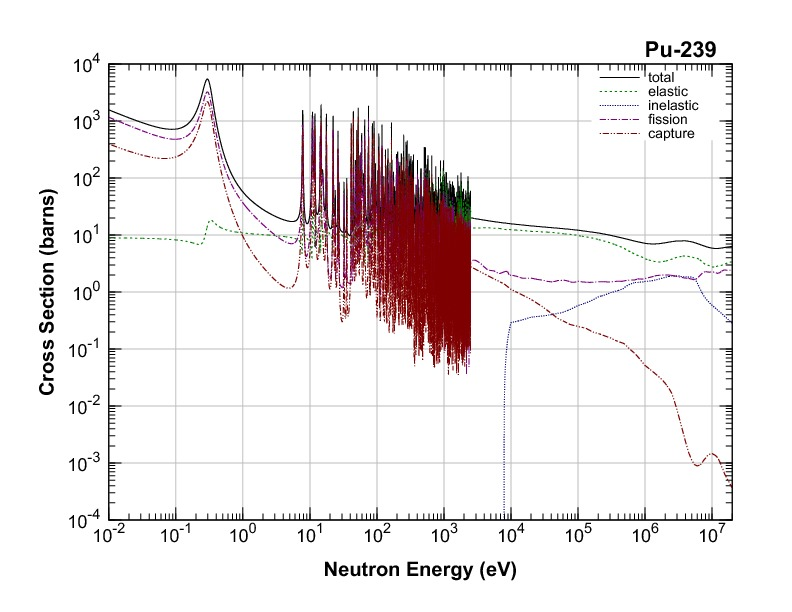
\includegraphics[width=0.75\textwidth]{pu239.cross.section.jpg}
%        \caption{}
    \end{figure}
\end{frame}


\begin{frame}{How do you choose materials?}
    \begin{columns}

        \begin{column}{0.75\textwidth}
            \begin{figure}
                \centering
                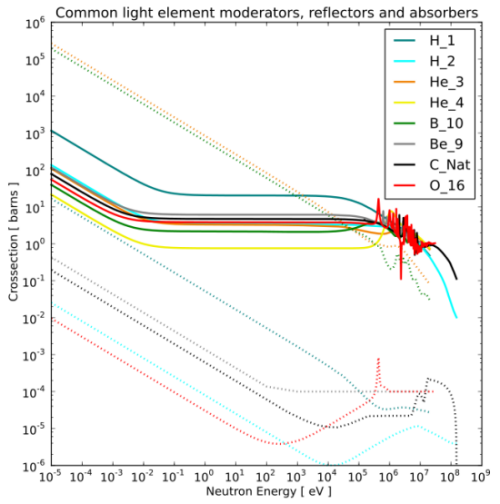
\includegraphics[width=0.70\textwidth]{moderators.jpg}
                %\caption{}
            \end{figure}
        \end{column}

        \begin{column}{0.25\textwidth}
            \begin{enumerate}[series=outerlist,topsep=0pt,itemsep=7pt,leftmargin=*,label=(\arabic*)]
                \item[]\small solid = scatter        
                \item[]\small dotted = absorption
            \end{enumerate}
        \end{column}

    \end{columns}
\end{frame}


\begin{frame}[plain]{}
    \centering\LARGE\textbf{Neutron fluence}
\end{frame}


\addtocounter{framenumber}{-1} 
\begin{frame}{How many neutrons/s that strike a target actually interact with target nuclei?}
    \begin{columns}[t]

        \begin{column}{0.55\textwidth}
            \begin{figure}
                \centering
                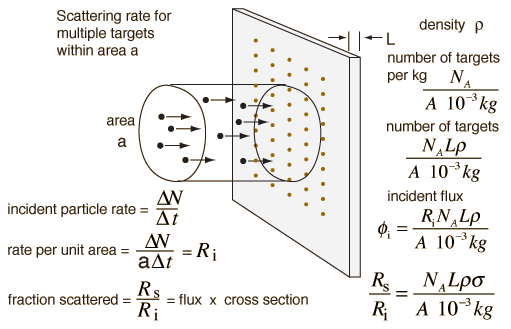
\includegraphics[width=0.95\textwidth]{flux.jpg}
                %\caption{}
            \end{figure}
        \end{column}

        \begin{column}{0.45\textwidth}
            \begin{equation}
                \small
                I[\frac{n}{cm^2 \cdot s}]=[\frac{n}{cm^3}] \cdot v[\frac{cm}{s}]
            \end{equation}

            \begin{equation}
                \small
                [\frac{n}{cm^3}] \cdot v[\frac{cm}{s}] \cdot a[cm^2]=\frac{n}{s}
            \end{equation}

            \begin{equation}
                \small
                nuclei_{tar} \equiv N[\frac{nuclei}{cm^3}] \cdot a[cm^2] \cdot L[cm]
            \end{equation}

            \begin{equation}
                \small
                \frac{interactions}{s} \equiv (\sigma I)(NaL)
            \end{equation}

            \vspace*{\fill}

            \begin{enumerate}[series=outerlist,topsep=0pt,itemsep=7pt,leftmargin=*,label=(\arabic*)]
                \item[]\small The cross section is the probability the neutron interacts with the nucleus
                \item[]\small Section 3.2, example 3.1 
            \end{enumerate}
        \end{column}

    \end{columns}
\end{frame}


\begin{frame}{Then we can define the mean free path}
    \begin{enumerate}[series=outerlist,topsep=0pt,itemsep=21pt,leftmargin=*,label=(\arabic*)]
        \item[]First, macroscopic cross section is --
    \end{enumerate}

    \vspace*{\fill}

    \begin{equation}
        \LARGE
        \Sigma [cm^{-1}] N \sigma = \frac{\rho N_A}{A}
    \end{equation}

    \vspace*{\fill}

    \begin{enumerate}[series=outerlist,topsep=0pt,itemsep=21pt,leftmargin=*,label=(\arabic*)]
        \item[]Then mean free path is --
    \end{enumerate}

    \vspace*{\fill}

    \begin{equation}
        \LARGE
        \lambda \equiv \Sigma^{-1} \; [cm]
    \end{equation}

    \vspace*{\fill}

    \begin{enumerate}[series=outerlist,topsep=0pt,itemsep=11pt,leftmargin=*,label=(\arabic*)]
        \item[]Expected value of distance between interactions
        \item[]Then the interaction rate is --
    \end{enumerate}

    \vspace*{\fill}

    \begin{equation}
        \LARGE
        R_X = \phi \Sigma_X
    \end{equation}

\end{frame}


\begin{frame}[plain]{}
    \centering\LARGE\textbf{Neutron flux}
\end{frame}


\addtocounter{framenumber}{-1} 
\begin{frame}{}
    \begin{columns}

        \begin{column}{0.75\textwidth}
            \begin{figure}
                \centering
                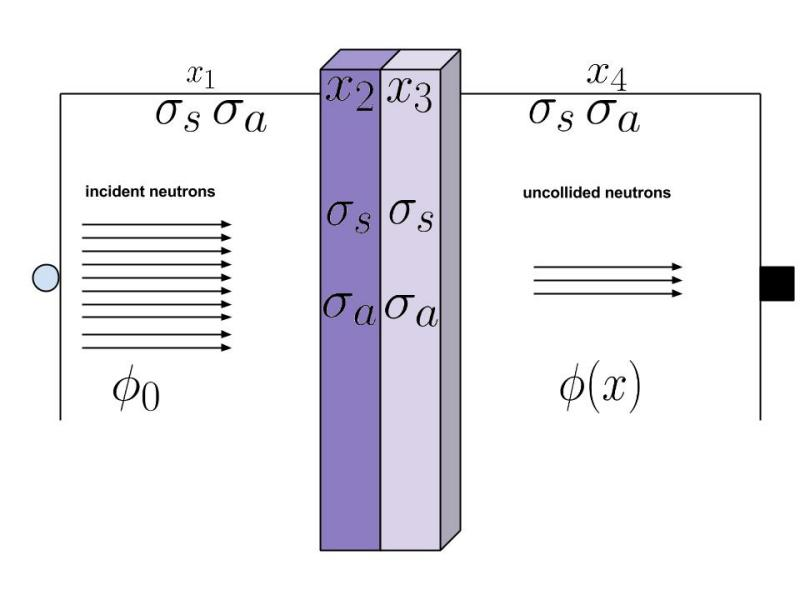
\includegraphics[width=0.95\textwidth]{shielding.jpg}
                %\caption{}
            \end{figure}
        \end{column}

        \begin{column}{0.25\textwidth}
            \begin{enumerate}[series=outerlist,topsep=0pt,itemsep=7pt,leftmargin=*,label=(\arabic*)]
                \item[]\small Which flux is larger?
                \item[]\small Point source
                \item[]\small Isotropic
            \end{enumerate}
        \end{column}

    \end{columns}
\end{frame}


\begin{frame}{Uncollided flux decreases exponentially with distance}

    \begin{equation}
        \LARGE
        -d\phi = \Sigma_t \phi dx
    \end{equation}

    \vspace*{\fill}

    \begin{equation}
        \LARGE
        -\frac{d\phi}{\phi} = \Sigma_t dx
    \end{equation}

    \vspace*{\fill}

    \begin{enumerate}[series=outerlist,topsep=0pt,itemsep=11pt,leftmargin=*,label=(\arabic*)]
        \item[]Probability a neutron interacts in dx
    \end{enumerate}

    \vspace*{\fill}

    \begin{equation}
        \LARGE
        \phi(x) = \phi_0 e^{-\Sigma_t x}
    \end{equation}

    \vspace*{\fill}

    \begin{enumerate}[series=outerlist,topsep=0pt,itemsep=11pt,leftmargin=*,label=(\arabic*)]
        \item[]Probability a neutron does not interact in x
    \end{enumerate}
\end{frame}


\begin{frame}{It's the same for gamma rays}
    \begin{enumerate}[series=outerlist,topsep=0pt,itemsep=11pt,leftmargin=*,label=(\arabic*)]
        \item[]Shielding is material density dependent
    \end{enumerate}

    \vspace*{\fill}

    \begin{equation}
        \LARGE
        \phi(x) = \phi_0 e^{-\mu x}
    \end{equation}

    \vspace*{\fill}

    \begin{enumerate}[series=outerlist,topsep=0pt,itemsep=11pt,leftmargin=*,label=(\arabic*)]
        \item[]Look up mass attenuation coefficient
    \end{enumerate}

    \vspace*{\fill}

    \begin{equation}
        \LARGE
        \frac{\mu}{\rho} \; [\frac{cm^2}{g}]
    \end{equation}

    \vspace*{\fill}

    \begin{enumerate}[series=outerlist,topsep=0pt,itemsep=11pt,leftmargin=*,label=(\arabic*)]
        \item[]Then just multiply mass attentuation by material density
    \end{enumerate}
\end{frame}


\begin{frame}[plain]{}
    \begin{figure}
        \centering
        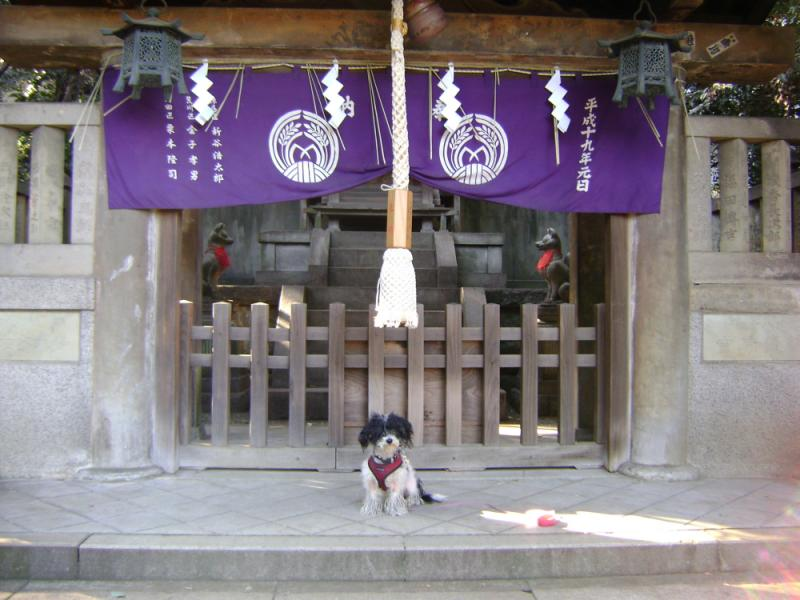
\includegraphics[width=0.75\textwidth]{final.jpg}
%        \caption{}
    \end{figure}
\end{frame}


%%%%%%%
%\begin{frame}{}
%    \begin{columns}
%
%        \begin{column}{0.50\textwidth}
%            \begin{enumerate}[series=outerlist,topsep=0pt,itemsep=21pt,leftmargin=*,label=(\arabic*)]
%                \item[]
%                \item[]
%            \end{enumerate}
%        \end{column}
%
%        \begin{column}{0.50\textwidth}
%            \begin{enumerate}[series=outerlist,topsep=0pt,itemsep=21pt,leftmargin=*,label=(\arabic*)]
%                \item[]
%                \item[]
%            \end{enumerate}
%        \end{column}
%
%    \end{columns}
%\end{frame}

%    \begin{figure}
%        \centering
%        \includegraphics[width=0.75\textwidth]{wsc.png}
%        \caption{\acs{wsc}}
%    \end{figure}


%\begin{frame}{References}
%    \bibliographystyle{nsf}
%    \footnotesize
%    \bibliography{references}
%\end{frame}
%%%%%%%


\end{document}
